\documentclass{llncs}
%%%%%%%%%%%%%%%%%%%%%%%%%%%%%%%%%%%%%%%%%%%%%%%%%%%%%%%%%%%
%% package sillabazione italiana e uso lettere accentate
\usepackage[utf8x]{inputenc}
\usepackage[english]{babel}
\usepackage[T1]{fontenc}
%%%%%%%%%%%%%%%%%%%%%%%%%%%%%%%%%%%%%%%%%%%%%%%%%%%%%%%%%%%%%

\usepackage{url}
\usepackage{xspace}
\usepackage{hyperref}
\usepackage{listings}
\usepackage{amsmath}
\usepackage{svg}
\makeatletter
%%%%%%%%%%%%%%%%%%%%%%%%%%%%%% User specified LaTeX commands.
%\usepackage{manifest}

\makeatother

%%%%%%%
 \newif\ifispdf
 \ifx\pdfoutput\undefined
 \ispdffalse % we are not running PDFLaTeX
 \else
 \pdfoutput=1 % we are running PDFLaTeX
 \ispdftrue
 \fi
%%%%%%%
% \usepackage[pdftex]{graphicx}
% \DeclareGraphicsExtensions{.pdf, .jpg, .tif,.png}
%%%%%%%%%%%%%%%

\newcommand{\action}[1]{\texttt{#1}\xspace}
\newcommand{\code}[1]{{\small{\texttt{#1}}}\xspace}
\newcommand{\codescript}[1]{{\scriptsize{\texttt{#1}}}\xspace}

% Cross-referencing
\newcommand{\labelsec}[1]{\label{sec:#1}}
\newcommand{\xs}[1]{\sectionname~\ref{sec:#1}}
\newcommand{\xsp}[1]{\sectionname~\ref{sec:#1} \onpagename~\pageref{sec:#1}}
\newcommand{\labelssec}[1]{\label{ssec:#1}}
\newcommand{\xss}[1]{\subsectionname~\ref{ssec:#1}}
\newcommand{\xssp}[1]{\subsectionname~\ref{ssec:#1} \onpagename~\pageref{ssec:#1}}
\newcommand{\labelsssec}[1]{\label{sssec:#1}}
\newcommand{\xsss}[1]{\subsectionname~\ref{sssec:#1}}
\newcommand{\xsssp}[1]{\subsectionname~\ref{sssec:#1} \onpagename~\pageref{sssec:#1}}
\newcommand{\labelfig}[1]{\label{fig:#1}}
\newcommand{\xf}[1]{\figurename~\ref{fig:#1}}
\newcommand{\xfp}[1]{\figurename~\ref{fig:#1} \onpagename~\pageref{fig:#1}}
\newcommand{\labeltab}[1]{\label{tab:#1}}
\newcommand{\xt}[1]{\tablename~\ref{tab:#1}}
\newcommand{\xtp}[1]{\tablename~\ref{tab:#1} \onpagename~\pageref{tab:#1}}

% Category Names
\newcommand{\sectionname}{Section}
\newcommand{\subsectionname}{Subsection}
\newcommand{\sectionsname}{Sections}
\newcommand{\subsectionsname}{Subsections}
\newcommand{\secname}{\sectionname}
\newcommand{\ssecname}{\subsectionname}
\newcommand{\secsname}{\sectionsname}
\newcommand{\ssecsname}{\subsectionsname}
\newcommand{\onpagename}{on page}

\newcommand{\xauthA}{Luca Mella}
\newcommand{\xauthB}{NameB StudentB}
\newcommand{\xauthC}{NameC StudentC}
\newcommand{\xfaculty}{II Faculty of Engineering}
\newcommand{\xunibo}{Alma Mater Studiorum -- University of Bologna}
\newcommand{\xaddrBO}{viale Risorgimento 2}
\newcommand{\xaddrCE}{via Venezia 52}
\newcommand{\xcityBO}{40136 Bologna, Italy}
\newcommand{\xcityCE}{47521 Cesena, Italy}


\begin{document}

\title{Class Project Report\\Metodi e Modelli per il Supporto alle Decisioni\\A.A. 2012/2013}

\author{\xauthA}

\institute{
\xunibo\\\xaddrCE, \xcityCE\\\email\ luca.mella@studio.unibo.it
}

\maketitle

\lstset{frame=lrb,xleftmargin=\fboxsep , xrightmargin=-\fboxsep}

%===========================================================================
\section{Obiettivi}
\labelsec{obiettivi}

Lo scopo del progetto è l'implementazione dell'algoritmo proposto in \cite{YANASSE2000} per ottenere le $K$ migliori soluzioni di un problema di \emph{Knapsack} ad una dimensione. Tale problema è detto \emph{Knapsack K-Best Problem} (\emph{KKP}).

\subsection{Piano di Lavoro}
\labelssec{piano}

Il progetto è stato articolato nelle seguenti macro-attività:

  \begin{enumerate}
    \item Prototipazione dell'algoritmo in \emph{Python}.
    \item Supporto alla risoluzione di librerie di problemi generate con il generatore sviluppato da \emph{Galassi e Leardini}.
    \item Implementazione dell'algoritmo in \emph{C++}.
    \item Documentazione e visualizzazione dati.
  \end{enumerate}

\section{Algoritmo per KKP}
\labelsec{algoritmo}

Il problema della determinazione delle $K$ migliori soluzioni del problema di knapsack può essere espresso come: 

\begin{equation} 
\begin{split}  
 C_{1 \times n} \cdot X_{n \times{} 1} = & z = \sum_{i=1}^{n} c_i X_i  
\\  X_k , z_k  \  with \  &  k \in 1 \dots K \  such \ that 
\\  X_1 , z_1 \mid & max \( \sum_{i=1}^{n} c_i x_{i}^{1} \) 
\\  X_2 , z_2 \mid & max \( \sum_{i=1}^{n} c_i x_{i}^{2} \) \  with \  X_2 \neq X_1 
\\  X_3 , z_3 \mid & max \( \sum_{i=1}^{n} c_i x_{i}^{3} \) \  with \  X_3 \neq X_2, \  X_3 \neq X_1 
\\ \cdots
\\ X_K, z_K \mid & max \( \sum_{i=1}^{n} c_i x_{i}^{K} \) \ such that \  X_K \neq X_{j} \  with \  j \in 1..K-1 
\\ \sum_{i=1}^n a_ix_i \le b 
\\ b, x_i,a_i \in \mathbb{N}_0 \end{split}
\end{equation}


Dove $K$ è il numero delle migliori soluzioni da determinare, $n$ è il numero degli oggetti considerati nel problema, $b$ è la capacità associata al knapsack, $x_i$ rappresentano le variabili decisionali associate agli oggetti del problema, $X_k$ il vettore di variabili decisionali associati alla $k$-esima soluzione, $a_i$ rappresentano i pesi, $c_i$ il profitto degli oggetti e $z_k$ il valore associato alla della $k$-esima soluzione determinata dal vettore di variabili decisionali $X_k$. 

L'algoritmo proposto in \cite{YANASSE2000} risolve il $KKP$ effettuando due distinti step enumerativi con complessità $O(Knb)$ nel tempo e $O(nb)$ in memoria in quanto viene utilizzata una come struttura dati di supporto 
una matrice $M_{b \times n }$.

\subsection{Enumerazione Forward}
\labelssec{forward}

Il primo step per la determinazione delle $K$ migliori soluzioni è popolare la matrice di supporto con i profitti $c_i$ associati alle variabili (\emph{ramification of supernodes}). La particolarità della matrice di supporto, ovvero la codifica dei pesi associati ad ogni elemento in una delle sue dimensioni, fa si di poter aggiornare i profitti consistentemente alle variabili in soluzione garantendo il rispetto dei vincoli di peso.

La matrice è costruita in mode che in ogni sua riga siano presenti al massimo le $n$ migliori soluzioni aventi peso uguale al valore dell'indice della riga stessa. Una volta popolata in accordo all'algoritmo proposto in \cite{YANASSE2000} (\emph{build initial $K$ best}) è possibile determinare il valore della migliore soluzione e di altre $K-1$ soluzioni qualitativamente soddisfacenti.

Tali soluzioni sono poste in una lista ed ordinate in base al loro profitto.

\subsection{Enumerazione Backward} 
\labelssec{backward}

L'enumerazione backward ha due principali scopi: ricostruire i valori delle variabili decisionali ed esplorare soluzioni alternative.

Nella parte di algoritmo denominata \emph{backtracking} si naviga all'indietro la matrice di supporto partendo da una qualsiasi soluzione. Sottraendo al costo della soluzione il costo dell'ultima variabile che è stata inserita in tale soluzione si ottiene l'indice della nuova riga da dove si è calcolato il valore della soluzione in fase \emph{forward}. Durante questo processo vengono incrementati i valori delle variabili decisionali relative alle variabili inserite in soluzione, inoltre viene mantenuta aggiornata una variabile accumulatore che contiene la componente di profitto della soluzione attribuita alle celle che si è attraversato durante la navigazione backward.
Questa componente di profitto ha un ruolo importante nella seconda fase dell'enumerazione backward, ovvero la \emph{ricerca di soluzioni alternative}.
Ad ogni passo compiuto all'indietro si cercano soluzioni alternative di profitto maggiore all'interno della riga che si sta analizzando (\emph{search alternative solution}), una volta localizzata tale soluzione si procede ad una ulteriore fase di \emph{backtracking} per ricostruire i valori delle variabili decisionali. 

Tale soluzione però non è ancora di buona qualità in quanto è noto che partendo da quella stessa riga della matrice di supporto (ovvero da quello stesso peso) si possono raggiungere profitti migliori unendo alla nuova soluzione trovata quella dal quale si era partiti a cercare soluzioni alternative. 
In altre parole si ottiene una soluzione di buona qualità aggiungendo alle variabili decisionali della soluzione alternativa le variabili decisionali ricostruite nella soluzione dalla quale si è cominciata la ricerca di ulteriori soluzioni.  

Tale processo termina dopo la ricostruzione delle variabili decisionali in ogni soluzione presente nella lista. 


\section{Implementazione}
\labelsec{implementazione}

L'algoritmo è stato in prima istanza prototipato in \emph{Python} ed in seguito è stato implementato in \emph{C++} per ottenere migliori prestazioni.

La compilazione della libreria e del tool a linea di comando avviene attraverso \emph{CMake}, dal quale è possibile generare soluzioni \emph{Visual Studio} o progetti \emph{Makefile} per Linux e Windows. Per la documentazione del codice si è adottato \emph{Doxygen}. Il progetto completo è disponibile su \emph{GitHub} \url{https://github.com/luca-m/kbest}.

\subsection{Risultati}
\labelssec{risultati}

Una veloce dimostrazione dell'algoritmo può essere ottenuta lanciando il tool a linea di comando con il parametro \emph{--sample} il quale risolverà il problema d'esempio riportato in \cite{YANASSE2000}, ulteriori dettagli sull'utilizzo del tool sono disponibili nel file ``README.md''.

I tempi di computazione registrati sono stati ottenuti risolvendo $400$ instanze del KP con $K \in \{ 10,30,50,70,90,110,130,150 \}$, quindi $3200$\footnote{I successivi grafici riportano solo le istanze che che rientrano nel secondo e terzo quartile} istanze del KKP. Le istanze sono state generate utilizzando il generatore fornito da \emph{Galassi e Leardini}, basato sul lavoro pubblicato nell' articolo \cite{Pisinger94}. Sono state utilizzate istanze di vario tipo: ``Strongly Correlated'', ``Weakly Correlated'', ``Uncorrelated'', ``Bounded Strongly Correlated'' e ``Subset Sum''. 

I grafici riportati in ~\ref{fig:time_by_b} riportano gli andamenti dei tempi di enumerazione in funzione della capacità, in ~\ref{fig:time_by_k_fw}~\ref{fig:time_by_k_bw} sono invece in funzione di $K$. Infine in \ref{fig:time_by_nbk_fw}~\ref{fig:time_by_nbk_bw} sono riportati gli andamenti dei tempi in funzione di numero di variabili $n$, capacità $b$ e parametro $K$. In questi ultimi è possibile notare come la ricerca forward sia sensibilmente influenzata dai $b$ e $n$, mentre la ricerca backward lo sia maggiormente rispetto al parametro $K$.

\begin{figure}[!hb]
  \centering

  \begin{minipage}{0.35\linewidth} 
  \raggedleft
  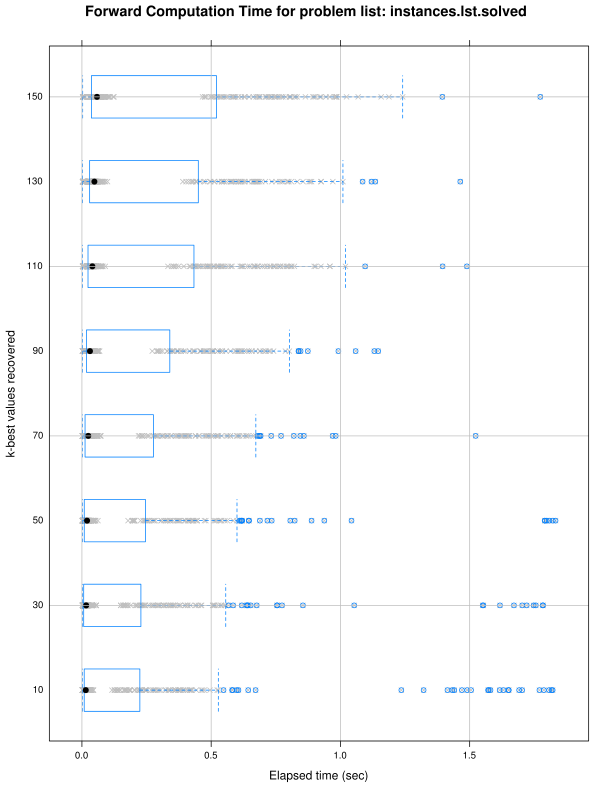
\includegraphics[width=6.4cm]{img/graph_all-time_by_k_fw.pdf}
  \caption{Tempo di enumerazione forward al variare di $K$}
  \label{fig:time_by_k_fw}
 \end{minipage}
 \hspace{2.5cm}
 \begin{minipage}{0.35\linewidth}
  \raggedright  
  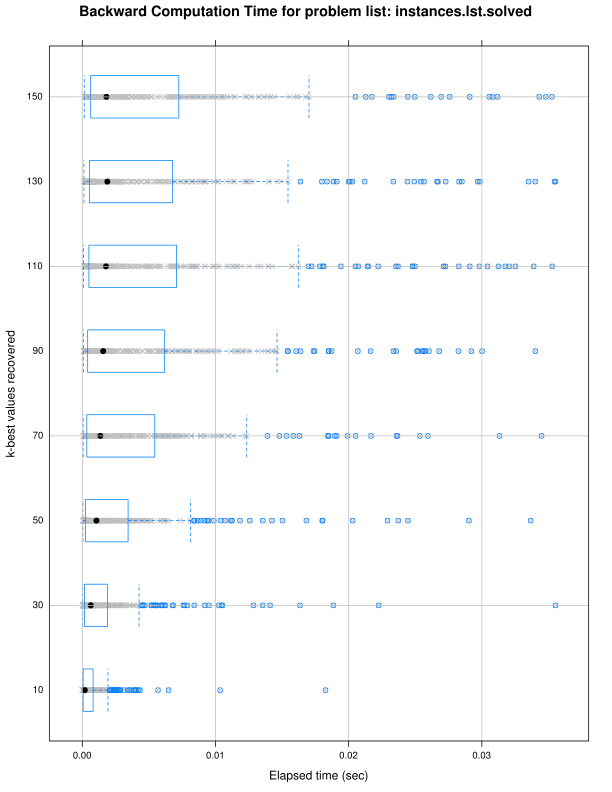
\includegraphics[width=6.4cm]{img/graph_all-time_by_k_bw.pdf}
  \caption{Tempo di enumerazione backward al variare di $K$}
  \label{fig:time_by_k_bw}
  \end{minipage}
  
\end{figure}

\newpage

\begin{figure}[!h]
  \centering
  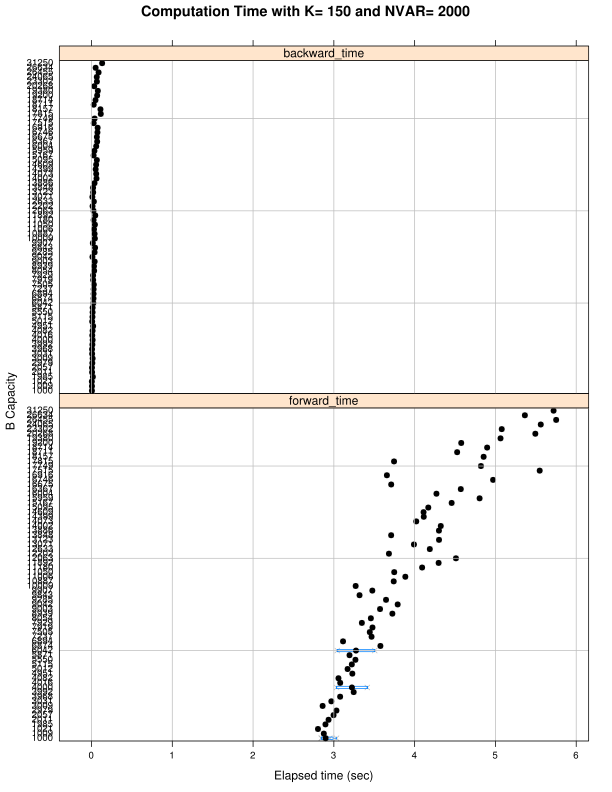
\includegraphics[width=12cm]{img/graph_all-time_by_b.pdf}.
  \caption{Tempi di soluzione con $K$ e numero di variabili fisso}
  \label{fig:time_by_b}
\end{figure}

\newpage

\begin{figure}[!h]
  \centering
  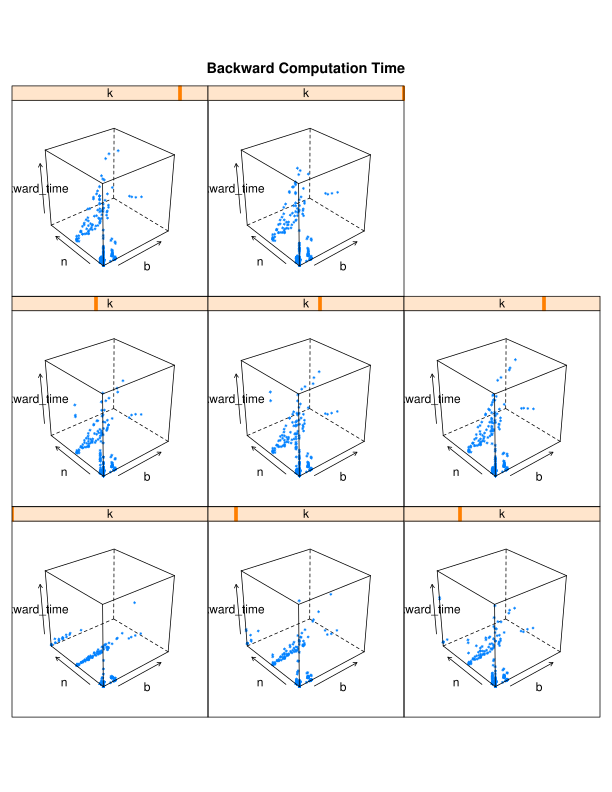
\includegraphics[width=12cm]{img/graph_all-time_by_nbk_bw.pdf}
  \caption{Tempo di enumerazione backward al variare di $K$, $b$ e $n$}
  \label{fig:time_by_nbk_bw}
\end{figure}

\newpage

\begin{figure}[!h]
  \centering
  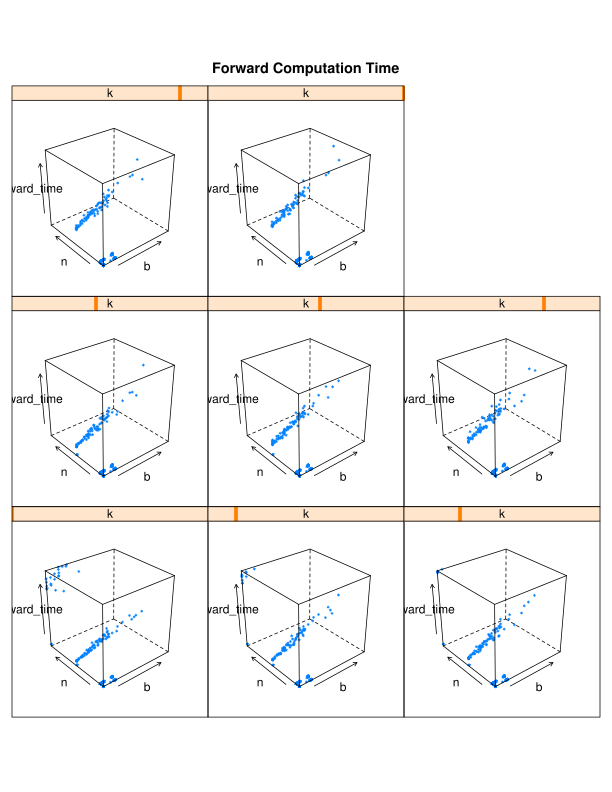
\includegraphics[width=12cm]{img/graph_all-time_by_nbk_fw.pdf}
  \caption{Tempo di enumerazione forward al variare di $K$, $b$ e $n$}
  \label{fig:time_by_nbk_fw}

\end{figure}

\newpage
\bibliographystyle{plain}
\bibliography{biblio} 
\end{document}













